\documentclass{article}

\usepackage{xcolor}
\usepackage{graphicx}
\usepackage{amsfonts, amsmath}

\begin{document}
\section{Experiments}
The explicit computations of the $(4, 2)$-Gromov-Wasserstein distance between
Euclidean spheres provides a helpful tool for benchmarking common optimal
transport packages. The authors are aware of two well-known and commonly used
python implementations of optimal transport solvers: Python Optimal Transport
(POT) \textcolor{blue}{CITE} and Optimal Transport Tools (OTT)
\textcolor{blue}{CITE}. These package implement two of the common methods for
computing the Gromov-Wasserstein distance--either with entropic regularization
(as with OTT) or without (as implemented in POT).\footnote{In fact, POT
provides implementations of both solving techniques, but we include OTT, which
only provides the regularized solver, since it is faster \textcolor{blue}{CITE}
because of its JAX implementation.} All experiments and their results are
available at the Github repository, \textcolor{blue}{CITE}.

The goal of this section is to benchmark various sampling methods and the
number of samples required to obtain accurate estimates of the
Gromov-Wasserstein distance while also understanding the accuracy of the
various solvers.

We run two sorts of experiments. First, we will examine how the number of
samples relates to the choice of a regularized or non-regularized solver.
Second, we will fix the number of samples and vary the dimensionality of the
spheres.

\subsection{Varied points experiment}

In this experiment, we fix the dimensions of both spheres and vary the number
of samples we draw from each one. For each number of points, we run $20$ trials
of each sampling method and Gromov-Wasserstein solver for each number of
samples between $10$ and $200$ in increments of $10$ (inclusive). The plotted
lines are the mean values estimated from the $20$ trials, while the shaded area
includes the central $80\%$ of samples.

\begin{figure}[hb]
    \centering
    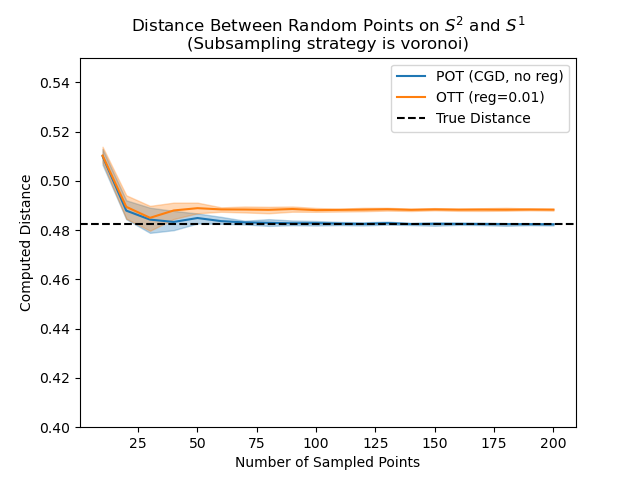
\includegraphics[width=0.3\linewidth]{../plots_same_axis/voronoi_trials/n_20_d_2_d1.png}
    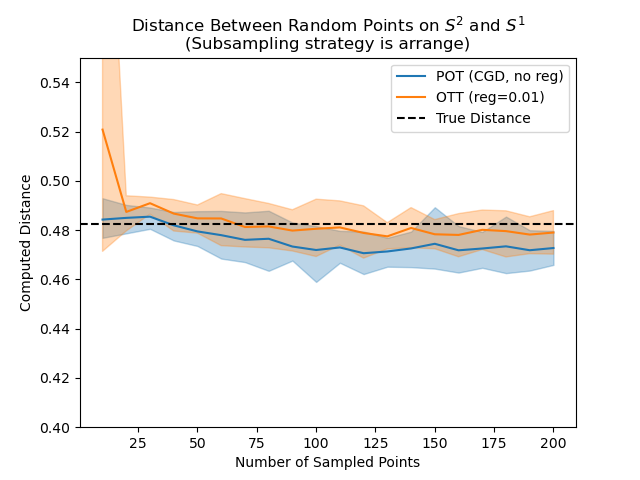
\includegraphics[width=0.3\linewidth]{../plots_same_axis/arrange_trials/n_20_d_2_d1.png}
    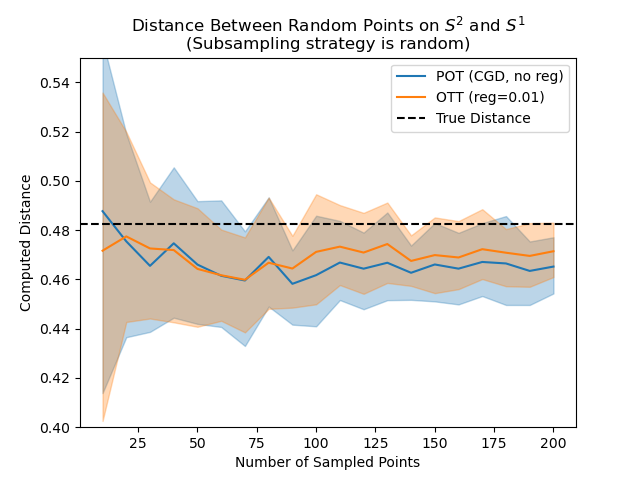
\includegraphics[width=0.3\linewidth]{../plots_same_axis/random_trials/n_20_d_2_d1.png}
    \caption{Estimating the Gromov-Wasserstein distance between $\mathbb{S}^2_E$ and $\mathbb{S}^1_E$.}
\end{figure}

\begin{figure}[hb]
    \centering
    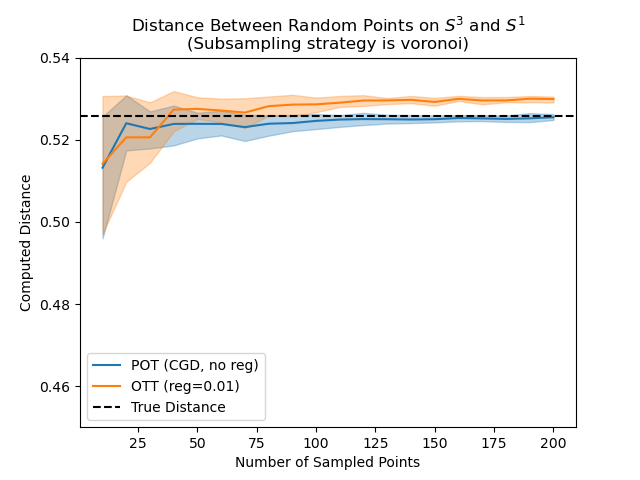
\includegraphics[width=0.3\linewidth]{../plots_same_axis/voronoi_trials/n_20_d_3_d1.png}
    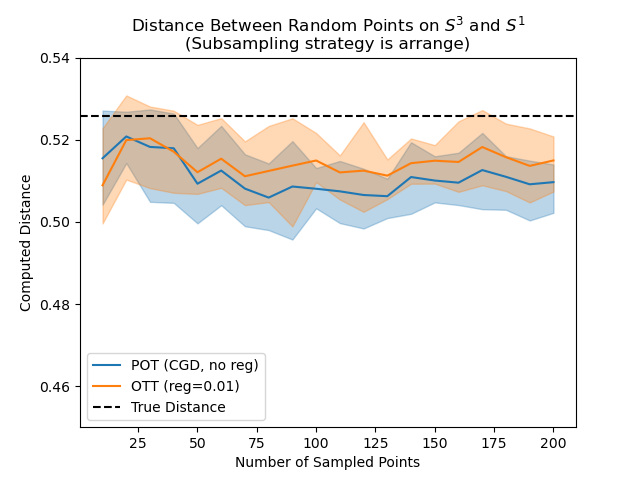
\includegraphics[width=0.3\linewidth]{../plots_same_axis/arrange_trials/n_20_d_3_d1.png}
    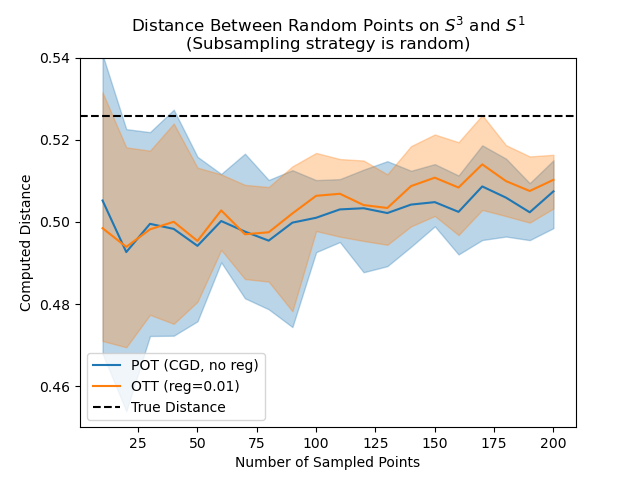
\includegraphics[width=0.3\linewidth]{../plots_same_axis/random_trials/n_20_d_3_d1.png}
    \caption{Estimating the Gromov-Wasserstein distance between $\mathbb{S}^3_E$ and $\mathbb{S}^1_E$.}
\end{figure}

\begin{figure}[hb]
    \centering
    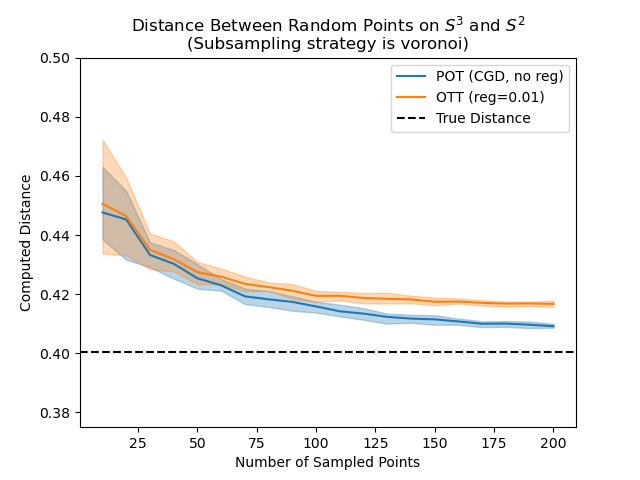
\includegraphics[width=0.3\linewidth]{../plots_same_axis/voronoi_trials/n_20_d_3_d2.png}
    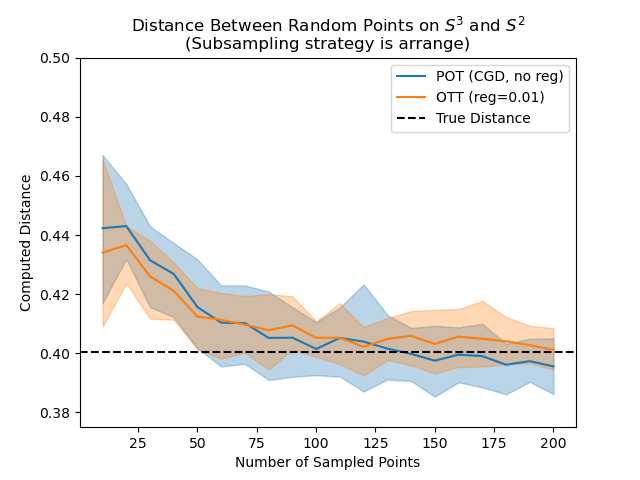
\includegraphics[width=0.3\linewidth]{../plots_same_axis/arrange_trials/n_20_d_3_d2.png}
    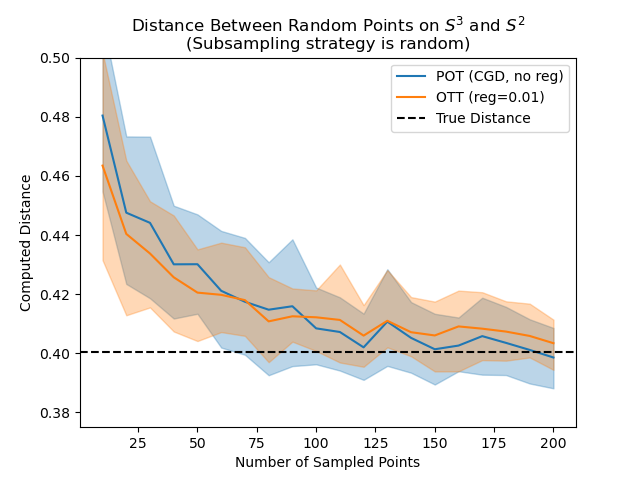
\includegraphics[width=0.3\linewidth]{../plots_same_axis/random_trials/n_20_d_3_d2.png}
    \caption{Estimating the Gromov-Wasserstein distance between $\mathbb{S}^3_E$ and $\mathbb{S}^2_E$.}
\end{figure}

\subsection{Varied dimensions experiment}
In this experiment, we fixed the number of samples taken at $100$ and varied
the dimensions of the two spheres, the solver method, and subsampling method.

Using the results of the trials for fixed sphere dimensions, $m$ and $n$,
$\hat{d}^i_{m, n}$, where $i = 1, \cdots, n_\textrm{trials}$, we estimated the
true distance,
\[ d_{m, n} \approx \hat{d}_{m, n} =
    \frac{1}{n_\textrm{trials}}\sum_{i=1}^{n_\textrm{trials}} \hat{d}^i_{m, n}.
\]

We then recorded the relative error of this estimator: $\textrm{relative
error}_{m, n} = \frac{\hat{d}_{m, n} - d_{m, n}}{d_{m, n}}$. Each of these
values is recorded in the corresponding entry of the heatmap.

\end{document}